
We define the following sets of monomorphisms to facilitate the discussion of the termination criterion. They are almost identical to those defined in Notation~\ref{subgraph_counting:notation:mono_sets}. 
\begin{notation}
    \label{antipattern:notation:mono_sets}
  Let \( \mathcal{X}\) be a ruler-graph with underlying graph $X$. The disjoint union of two sets \( S \) and \( S' \) is denoted by \( S \uplus S' \). Let \( X, A, B, G \) be graphs, and let \( \alpha \mathop{\colon} A \mathop{\to} G \) and \( \beta \mathop{\colon} B \mathop{\to} G \) be morphisms as illustrated below:
  \begin{center}
        \resizebox{0.4\textwidth}{!}{
            \begin{tikzpicture}
            \node (X) at (-1.5,-1) {$X$};
            \node (B) at (2,0) {$A$}; 
            \node (C) at (0,2) {$B$}; 
            \node (D) at (0,0) {$G$}; 
            \draw [>->] (B) to node [above,label,pos=0.45] {$\alpha$} (D); 
            \draw [>->] (C) to node [right,label,pos=0.45] {$\beta$} (D);
            \draw [>->,dashed] (X) to node [above,label,pos=0.45] {$\iota$} (D);
            \draw [>->,dashed] (X) to node [below,label,pos=0.45] {$\zeta$} (B);
            \draw [>->,dashed] (X) to node [above,label,pos=0.45] {$\eta$} (C);
        \end{tikzpicture}
        }
    \end{center}
     We define the following sets of monomorphisms from $X$ into $G$ based on their interaction with $\alpha$ and $\beta$:    
    \begin{align*}
        \operatorname{Mono}(\mathcal{X},G) &= \operatorname{Mono}(X,G), 
        \\
        \operatorname{Mono}(\mathcal{X},G,\alpha) &= \left\{ \iota \mathop{\colon} X \rightarrowtail G 
        \;\middle|\; 
        \exists \zeta \mathop{\colon} X \rightarrowtail A.\, \iota \mathop{=} \zeta \mathop{\star} \alpha \right\}, 
        \\
        \operatorname{Mono}(\mathcal{X},G,\mathop{\lnot} \alpha) &= \left\{ \iota \mathop{\colon} X \rightarrowtail G 
        \;\middle|\; 
        \nexists \zeta \mathop{\colon} X \rightarrowtail A.\, \iota \mathop{=} \zeta \mathop{\star} \alpha \right\}, 
        \\
        \operatorname{Mono}(\mathcal{X},G,\mathop{\lnot} \alpha, \beta) &= \left\{ 
            \iota \mathop{\colon} X \rightarrowtail G \;\middle|\; 
                \begin{aligned}  
                    &(\nexists \zeta \mathop{\colon} X \rightarrowtail A.\, \iota \mathop{=} \zeta \mathop{\star} \alpha) \\ 
                    &\land (\exists \eta \mathop{\colon} X \rightarrowtail B.\, \iota \mathop{=} \eta \mathop{\star} \beta)
                \end{aligned}
        \right\},
        \\
        \operatorname{Mono}(\mathcal{X},G,\mathop{\lnot} \alpha, \mathop{\lnot} \beta) &= \left\{ 
            \iota \mathop{\colon} X \rightarrowtail G \;\middle|\; 
                \begin{aligned}
                    &(\nexists \zeta \mathop{\colon} X \rightarrowtail A.\, \iota \mathop{=} \zeta \mathop{\star} \alpha) \\
                    &\land (\nexists \eta \mathop{\colon} X \rightarrowtail B.\, \iota \mathop{=} \eta \mathop{\star} \beta)
                \end{aligned}
        \right\}.
    \end{align*}
    For a set $\operatorname{Mono}(\mathcal{X},\dots)$, we write $\operatorname{Mono}(\mathcal{X},\dots)_{\operatorname{NF}}$ for the subset of \( X \)-occurrences whose images are not included in any occurrence of the forbidden context if it exists, and  $\operatorname{Mono}(\mathcal{X},\dots)_{\operatorname{F}}$ for the subset of \( X \)-occurrences whose images are included in some occurrences of the forbidden context if it exists. 
\end{notation}
    Let $\mathcal{X}=(X,\mathcal{C})$ be a ruler-graph and \( \rho \mathop{=} (L \overset{l}{\leftarrowtail} K \overset{r}{\rightarrowtail} R) \) be a rule. 
    Consider the following DPO diagram:
    \begin{center}
        \resizebox{0.3\textwidth}{!}{
   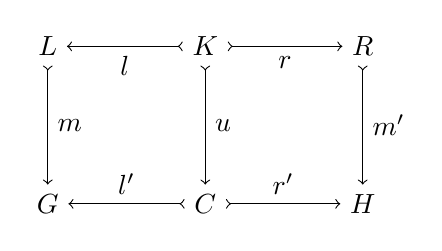
\begin{tikzpicture}
            % [node distance=15mm]
            \node (I) at (0,0) {$K$};
            \node (L)  at (-2,0) {$L$};
            \node (R)  at (2,0) {$R$};
            \node (G)  at (-2,-2) {$G$};
            \node (C)  at (0,-2) {$C$};
            \node (H)  at (2,-2) {$H$};
            \draw [>->] (I) to  node [midway,below] {$l$} (L);
            \draw [>->] (I) to  node [midway,below] {$r$} (R);
            \draw [>->] (L) to node [midway,right] {$m$} (G);
            \draw [>->] (I) to  node [midway,right] {$u$} (C);
            \draw [>->] (R) to  node [midway,right] {$m'$} (H);
            \draw [>->] (C) to node [midway,above] {$l'$} (G);
            \draw [>->] (C) to node [midway,above] {$r'$} (H);
            % \node [at=($(I)!.5!(G)$)] {\normalfont PO};
            % \node [at=($(I)!.5!(H)$)] {\normalfont PO};
        \end{tikzpicture}
        }
    \end{center}

The set $\operatorname{Mono}(\mathcal{X},G)_{\operatorname{NF}}$ 
decomposes into a union of three disjoint subsets:
\begin{itemize}
    \item $\operatorname{Mono}(\mathcal{X},G,m)_{\operatorname{NF}}$,
    \item $\operatorname{Mono}(\mathcal{X},G,\mathop{\lnot} m, l')_{\operatorname{NF}}$,
    \item $\operatorname{Mono}(\mathcal{X},G,\mathop{\lnot} m, \mathop{\lnot} l')_{\operatorname{NF}}$.
\end{itemize}
% $$
%     \operatorname{Mono}(\mathcal{X},G,m)_{\operatorname{NF}}
%     \uplus
%     \operatorname{Mono}(\mathcal{X},G,\mathop{\lnot} m, l')_{\operatorname{NF}} 
%     \uplus
%     \operatorname{Mono}(\mathcal{X},G,\mathop{\lnot} m, \mathop{\lnot} l')_{\operatorname{NF}}.
% $$
Similarly, the set
 $\operatorname{Mono}(\mathcal{X},H)_{\operatorname{NF}}$ decomposes into a union of three disjoint subsets:
 \begin{itemize}
    \item $\operatorname{Mono}(\mathcal{X},H,m')_{\operatorname{NF}}$,
    \item $\operatorname{Mono}(\mathcal{X},H,\mathop{\lnot} m', r')_{\operatorname{NF}}$,
    \item $\operatorname{Mono}(\mathcal{X},H,\mathop{\lnot} m', \mathop{\lnot} r')_{\operatorname{NF}}$.
 \end{itemize}
\noindent
Thus, the following equality holds:
\begin{flalign}
    &\card{\operatorname{Mono}(\mathcal{X},G)_{\operatorname{NF}}} \mathop{-} 
    \card{\operatorname{Mono}(\mathcal{X},H)_{\operatorname{NF}}} \nonumber
    \\=
    &(\card{\operatorname{Mono}(\mathcal{X},G,m)_{\operatorname{NF}}} 
        \mathop{-}  
    \card{\operatorname{Mono}(\mathcal{X},H,m')_{\operatorname{NF}}}) 
   \mathop{+} \nonumber
    \\
    &(
        \card{\operatorname{Mono}(\mathcal{X},G,\mathop{\lnot} m, l')_{\operatorname{NF}}}
             \mathop{-} 
        \card{\operatorname{Mono}(\mathcal{X},H,\mathop{\lnot} m', r')_{\operatorname{NF}}})\mathop{+} \nonumber \\ 
    &(
        \card{\operatorname{Mono}(\mathcal{X},G,\mathop{\lnot} m, \mathop{\lnot} l')_{\operatorname{NF}}} 
            \mathop{-} 
        \card{\operatorname{Mono}(\mathcal{X},H,\mathop{\lnot} m', \mathop{\lnot} r')_{\operatorname{NF}}} 
    ).\nonumber
\end{flalign}
In the remainder of this section, we suppose that $\rho^{-1}$ is $F$-non-increasing if $\mathcal{C} \mathop{=} \set{f:X \mathop{\rightarrowtail} F}$ and that $\rho$ and $\rho^{-1}$ are $X$-non-increasing. To estimate $\card{\operatorname{Mono}(\mathcal{X},G)_{\operatorname{NF}}} \mathop{-} 
    \card{\operatorname{Mono}(\mathcal{X},H)_{\operatorname{NF}}}$, we establish the following lemmas.
% The following lemmas can be used to approximate $\card{\operatorname{Mono}(\mathcal{X},G)_{\operatorname{NF}}} \mathop{-} 
%     \card{\operatorname{Mono}(\mathcal{X},H)_{\operatorname{NF}}}$
\begin{lemma}
    \label{antipattern:lem:xglnotmlp_xhlnotmrp}
        Let \( \rho \mathop{=} (L \overset{l}{\leftarrowtail} K \overset{r}{\rightarrowtail} R) \) be a rule and $\mathcal{X}=(X,\mathcal{C})$ be a ruler-graph. 
        Suppose that $\rho^{-1}$ is $F$-non-increasing if $\mathcal{C} \mathop{=} \set{f:X \rightarrowtail F}$.
        The following inequality holds:
    $$\card{\operatorname{Mono}(\mathcal{X},G,\mathop{\lnot} m, l')_{\operatorname{NF}}} \geq
        \card{\operatorname{Mono}(\mathcal{X},H,\mathop{\lnot} m', r')_{\operatorname{NF}}}.$$
\end{lemma} 
\begin{lemma}
    \label{antipattern:lem:xglnotmlnotlp_xhlnotmrnotrp}
        Let \( \rho \mathop{=} (L \overset{l}{\leftarrowtail} K \overset{r}{\rightarrowtail} R) \) be a rule, and let $\mathcal{X}=(X,\mathcal{C})$ be a ruler-graph. Suppose that $\rho$ and $\rho^{-1}$ are $X$-non-increasing. We have
    $$ 
        \card{\operatorname{Mono}(\mathcal{X},G,\mathop{\lnot} m, \mathop{\lnot} l')_{\operatorname{NF}}} \geq
        \card{\operatorname{Mono}(\mathcal{X},H,\mathop{\lnot} m', \mathop{\lnot} r')_{\operatorname{NF}}}.
    $$
\end{lemma}
Under the assumptions of the above two lemmas, we obtain the following inequality:
 \begin{flalign*}
     \card{\operatorname{Mono}(\mathcal{X},G)_{\operatorname{NF}}} \mathop{-} 
     \card{\operatorname{Mono}(\mathcal{X},H)_{\operatorname{NF}}} 
     \geq
     \card{\operatorname{Mono}(\mathcal{X},G,m)_{\operatorname{NF}}} \mathop{-} \card{\operatorname{Mono}(\mathcal{X},H,m')_{\operatorname{NF}}}.
 \end{flalign*}

\begin{definition}
    \label{antipattern:def:gamma_l_rho_x}
    Let $\mathcal{X}=(X,\mathcal{C})$ be a ruler-graph, and let \( \rho \mathop{=} (L \overset{l}{\leftarrowtail} K \overset{r}{\rightarrowtail} R) \) be a rule.
    Define $\Gamma(\operatorname{Mono}(\mathcal{X},L)_{\operatorname{NF}})$ as the subset of $\operatorname{Mono}(\mathcal{X},L)_{\operatorname{NF}}$ consisting of $X$-occurrences whose images are not included in any occurrence of the forbidden context in $L$,
    but, in some rewriting step $G \mathop{\Rightarrow}_\rho^m H$, their images may possibly be included in some occurrence of the forbidden context in the host graph $G$.
    Formally,  $\Gamma(\operatorname{Mono}(\mathcal{X},L)_{\operatorname{NF}}) \mathop{=} \emptyset$ if $\mathcal{C} \mathop{=} \emptyset$, and if $\mathcal{C} \mathop{=} \set{f:X \rightarrowtail F}$, then a monomorphism $h_{XL}:X \rightarrowtail L$ is in $\Gamma(\operatorname{Mono}(\mathcal{X},L)_{\operatorname{NF}})$ if and only if the following hold:
    \begin{itemize}
        \item there does not exist $h_{FL}:F \rightarrowtail L$ such that $f \mathop{\star} h_{FL} \mathop{=} h_{XL}$, and
         \item  
         there are a graph $C$, a monomorphism $K \overset{u}{\rightarrowtail} C$, and the pushout $L \overset{m}{\rightarrowtail} G \overset{l'}{\leftarrowtail} C$ of $L \overset{l}{\leftarrowtail} K \overset{u}{\rightarrowtail} C$ such that
         there is a monomorphism $h_{FG} : F \rightarrowtail G$ satisfying
         $h_{XL} \mathop{\star} m \mathop{=} h_{XF} \mathop{\star} h_{FG}$. 
      \begin{center}
        \resizebox{0.4\textwidth}{!}{
            \begin{tikzpicture}
                    \node (k) at (0,1) {K};
                    \node (l) at (-2,1) {L};
                    \node (c) at (0,-1) {C};
                    \node (g) at (-2,-1) {G};
                    \node (x) at (-4,-2) {X};
                    \node (f) at (-2,-2) {F};
                    \draw[<-<]  (l) -- (k) node [midway,below] {$l$};
                    \draw[>->] (c) -- (g) node [midway, above] {$l'$};
                    \draw[>->] (l) -- (g) node[midway, right] {$m$};
                    \draw[>->] (k) -- (c) node[midway, left] {$u$};
                    \draw[>->] (x) -- (l) node[midway, left] {$h_{XL}$};
                    \draw[>->] (x) -- (f) node[midway, above] {$f$};
                    \draw[>->] (f) -- (g) node[midway, right] {$h_{FG}$};
                    \node () [at=($(l)!0.5!(c)$)] {$PO$};
                \end{tikzpicture}
         }
        \end{center}
    \end{itemize}
    We define $\Lambda(\mathcal{X},\rho) \overset{\operatorname{def}}{=} (\card{\operatorname{Mono}(\mathcal{X},L)_{\operatorname{NF}}} \mathop{-} 
    \card{\Gamma(\operatorname{Mono}(\mathcal{X},L)_{\operatorname{NF}})}) -
   \card{\operatorname{Mono}(\mathcal{X},R)_{\operatorname{NF}}}$ to improve readability.
%    \trackedtext{Intuitively, $\Lambda(\mathcal{X},\rho)$ is the number of $X$-occurrences in $L$ ...}
\end{definition}
Note that in the category \textbf{Graph}, the pushout of two arrows always exists~\cite[p.188]{corradini1997algebraic}. This justifies the existence of the pushout square in the second condition of the above definition.
Furthermore, since $X$ and the forbidden context (if exists) are finite graphs, $\Lambda(\mathcal{X},\rho)$ can be precisely computed. Consequently, it provides a lower bound for the change in the number of $X$-occurrences in a rewriting step using $\rho$, as shown in the following lemma whose proof is given in~\textsection~\ref{antipattern:proof:lem:xgm_xhmp_xl_xr}.

% \begin{lemma}
%     \label{lem:decomp_w_u}
%     \ \newline
%     \noindent
%     \begin{minipage}{0.7\textwidth}
%         Let $X$ be a ruler-graph. For a pushout square as shown on the right, we have 
%         % $\card{\operatorname{Mono}(X, B)} \mathop{=} \card{\operatorname{Mono}(X, D, \beta')}$ and $\card{\operatorname{Mono}(X, C, \mathop{\lnot} \beta)} \mathop{=} \card{\operatorname{Mono}(X, D, \mathop{\lnot} \beta', \alpha')}$.
%         \begin{flalign*}
%             \card{\operatorname{Mono}(X, B)} &= \card{\operatorname{Mono}(X, D, \beta')}
%             \\
%             \card{\operatorname{Mono}(X, C, \mathop{\lnot} \beta)} &= \card{\operatorname{Mono}(X, D, \mathop{\lnot} \beta', \alpha')}
%         \end{flalign*}
%     \end{minipage}
%     \hfill
%     \begin{minipage}{0.3\textwidth}
%         \hfill
%         \begin{tikzpicture}
%             \node (A) {$A$};
%             \node [below of=A] (B) {$B$}; 
%             \node [left of=A] (C) {$C$}; 
%             \node [left of=B] (D) {$D$}; 
%             \begin{scope}[nodes=rectangle]          
%             \draw [>->] (A) to node [right,label,pos=0.5] {$\alpha$} (B);
%             \draw [>->] (A) to node [above,label,pos=0.5] {$\beta$} (C);
%             \draw [>->] (B) to node [below,label,pos=0.45] {$\beta'$} (D); 
%             \draw [>->] (C) to node [left,label,pos=0.45] {$\alpha'$} (D);
%             \end{scope}
%         \end{tikzpicture}
%     \end{minipage} 
% \end{lemma}
% \begin{proof}
%     See the Appendix,~\autoref{proof:dcomp_w_u}.
%  \end{proof}
% \begin{lemma}
%     \label{lem:xgm_xhmp_xl_xr}
%     % If the number of $X$-occurrences that are not  included in any occurrences of forbidden context $F \mathop{\in} F_x$ in a $\rho$-rewriting step is predictable, then
%     $
%         \card{\operatorname{Mono}(\mathcal{X},G,m)_{\operatorname{NF}}} \mathop{-} 
%         \card{\operatorname{Mono}(\mathcal{X},H,m')_{\operatorname{NF}}} 
%         \mathop{\geq} 
%         \card{\operatorname{Mono}(X,L)} -
%         \card{\operatorname{Mono}(X,R)}
%     $
% \end{lemma}
% \begin{proof}
%     See the Appendix, \textsection~\ref{proof:lem:xgm_xhmp_xl_xr}.
%  \end{proof}

\begin{lemma}
    \label{antipattern:lem:xgm_xhmp_xl_xr}
     Let $\mathcal{X}$ be a ruler-graph, and let \( \rho \mathop{=} (L \overset{l}{\leftarrowtail} K \overset{r}{\rightarrowtail} R) \) be a rule. 
   We have
    \begin{flalign*}
        &\card{\operatorname{Mono}(\mathcal{X},G,m)_{\operatorname{NF}}} \mathop{-} 
        \card{\operatorname{Mono}(\mathcal{X},H,m')_{\operatorname{NF}}} 
        \geq
        \Lambda(\mathcal{X},\rho).
    \end{flalign*}
\end{lemma}
 Thus, by the unnumbered equation preceding Definition~\ref{antipattern:def:gamma_l_rho_x}, the following inequality holds:
 \begin{flalign}
         \card{\operatorname{Mono}(\mathcal{X},G)_{\operatorname{NF}}} \mathop{-} 
     \card{\operatorname{Mono}(\mathcal{X},H)_{\operatorname{NF}}} 
     \mathop{\geq} 
    \Lambda(\mathcal{X},\rho).
     \label{eq:mono_x_g_nf_mono_x_h_nf_geq}
 \end{flalign}
Consequently, we have  
\begin{flalign*}
    w_{s_\mathbb{X}}(G) \mathop{-} w_{s_\mathbb{X}}(H)
   \overset{\operatorname{def}}{=}&\sum_{\mathcal{X} \mathop{\in} \mathbb{X}}^{}s_\mathbb{X}(\mathcal{X}) \mathop{*} m_X(G) \mathop{-} \sum_{\mathcal{X} \mathop{\in} \mathbb{X}}^{}s_\mathbb{X}(\mathcal{X}) \mathop{*} m_X(H)
   \\
   \overset{\operatorname{def}}{=}&\sum_{\mathcal{X} \mathop{\in} \mathbb{X}}^{}s_\mathbb{X}(\mathcal{X}) \mathop{*} |\operatorname{Mono}(\mathcal{X},G)_{\operatorname{NF}}| \mathop{-} \sum_{\mathcal{X} \mathop{\in} \mathbb{X}}^{}s_\mathbb{X}(\mathcal{X}) \mathop{*} |\operatorname{Mono}(\mathcal{X},H)_{\operatorname{NF}}|
   \\
   =&\sum_{\mathcal{X} \mathop{\in} \mathbb{X}}^{}s_\mathbb{X}(\mathcal{X}) \mathop{*} \left( \card{\operatorname{Mono}(\mathcal{X},G)_{\operatorname{NF}}} \mathop{-} 
   \card{\operatorname{Mono}(\mathcal{X},H)_{\operatorname{NF}}} \right)
   \\
   \geq&\sum_{\mathcal{X} \mathop{\in} \mathbb{X}}^{}s_\mathbb{X}(\mathcal{X}) \mathop{*} \Lambda(\mathcal{X},\rho).
   \hspace{2cm} \text{by~\eqref{eq:mono_x_g_nf_mono_x_h_nf_geq}}
\end{flalign*} 
This proves the following key lemma of this section.
\begin{lemma}[Decreasing step]
    \label{antipattern:lem:w_g_geq_w_h_leq}
    Let $\rho \mathop{=} (L \overset{l}{\leftarrowtail} K \overset{r}{\rightarrowtail} R)$ be an injective DPO rewriting rule,
    \( \mathbb{X} \) a set of ruler-graphs,
    \( s_{\mathbb{X}} \mathop{\colon} \mathbb{X} \mathop{\to} \mathbb{N} \) a weight function,
    and \( G \mathop{\Rightarrow}_{\rho,\mathfrak{M}} H \) a rewriting step. 
    Suppose that for every \( \mathcal{X}=(X,\mathcal{C}) \mathop{\in} \mathbb{X} \), 
    % the number of $X$-occurrences that are not included in any occurrences of forbidden context $F \mathop{\in} F_x$ in a $\rho$-rewriting step is predictable,
    $\rho$ is $X$-non-increasing, and if $\mathcal{C}= \set{f:X \rightarrowtail F}$ then $\rho^{-1}$ is $X$-non-increasing and $F$-non-increasing. The following inequality holds:
     $$
        w_{s_\mathbb{X}}(G) \mathop{-} w_{s_\mathbb{X}}(H) 
        \mathop{\geq} 
        \sum_{\mathcal{X} \mathop{\in} \mathbb{X}}^{}s_\mathbb{X}(\mathcal{X}) \mathop{*} \Lambda(\mathcal{X},\rho).
    $$
\end{lemma}
Finally, our main result follows.
\begin{theorem}[Termination] 
    \label{antipattern:thm:termination_grs} 
    Let \(\mathcal{A}\) and \(\mathcal{B}\) be sets of injective DPO rewriting rules, $\mathbb{X}$ a set of ruler-graphs, and $s_\mathbb{X}$ a weight function. If the following hold:
    \begin{enumerate}
        \item  for every $\rho \mathop{\in} \mathcal{A} \mathop{\cup} \mathcal{B}$ and for every \( \mathcal{X} = (X, \mathcal{C}) \mathop{\in} \mathbb{X} \), 
        % the number of $X$-occurrences that are not included in any occurrences of the forbidden context $F \mathop{\in} F_x$ in a $\rho$-rewriting step is predictable,
        $\rho$ is $X$-non-increasing, and if $\mathcal{C}= \set{f:X \rightarrowtail F}$ then $\rho^{-1}$ is $X$-non-increasing and $F$-non-increasing, and
        % $\rho^{-1}$ is $F$-non-increasing if $\mathcal{X}= (X,f:X \rightarrowtail F)$ and, $\rho$ and $\rho^{-1}$ are $X$-non-increasing
        \item for every \(\rho \mathop{\in} \mathcal{A}\), we have
        % \( w_{s_\mathbb{X}}(lhs(\rho)) \mathop{>} w_{s_\mathbb{X}}(rhs(\rho)) \),
        $ \sum_{\mathcal{X} \mathop{\in} \mathbb{X}}^{}s_\mathbb{X}(\mathcal{X}) \mathop{*} 
            \Lambda(\mathcal{X},\rho) \mathop{>} 0 $, and
        \item for every \(\rho \mathop{\in} \mathcal{B}\), we have   
        % \( w_{s_\mathbb{X}}(lhs(\rho)) \mathop{\geq} w_{s_\mathbb{X}}(rhs(\rho)) \).
        $ 
            \sum_{\mathcal{X} \mathop{\in} \mathbb{X}}^{}s_\mathbb{X}(\mathcal{X}) \mathop{*} \Lambda(\mathcal{X},\rho) \mathop{\geq} 0 
        $.
    \end{enumerate}
    Then \(\mathop{\Rightarrow}_{\mathcal{A},\mathcal{M}}\) terminates relative to \(\mathop{\Rightarrow}_{\mathcal{B},\mathcal{M}}\).
\end{theorem}
\begin{remark}
    This work focuses on deriving sufficient conditions for termination, deferring the construction of ruler-graphs to future work.
\end{remark} 
